\documentclass[border=3pt]{standalone}
\usepackage[T1]{fontenc}
\usepackage[utf8]{inputenc}
\usepackage{lmodern}
\usepackage{amsmath,amssymb}
\usepackage{xcolor}
\usepackage{tikz}
\usepackage{fontawesome5}
\usepackage{ragged2e}
\usetikzlibrary{shapes,shapes.geometric,shapes.misc,arrows.meta,positioning,
                calc,fit,backgrounds,decorations.pathreplacing,
                decorations.markings,patterns,chains}
\usetikzlibrary{decorations.pathreplacing,decorations.markings}
\definecolor{primary}{HTML}{1A5276}
\definecolor{secondary}{HTML}{2E86C1}
\definecolor{accent}{HTML}{E74C3C}
\definecolor{lightbg}{HTML}{EBF5FB}
\definecolor{defbg}{HTML}{FDF2E9}
\definecolor{greenhl}{HTML}{27AE60}
\definecolor{purplehl}{HTML}{8E44AD}
\definecolor{goldhl}{HTML}{B7950B}
\definecolor{tealhl}{HTML}{117A65}
\definecolor{codebg}{HTML}{F4F6F7}
\definecolor{neutral}{HTML}{707B7C}
\definecolor{dom1}{HTML}{1F618D}
\definecolor{dom2}{HTML}{117864}
\definecolor{dom3}{HTML}{6C3483}
\definecolor{dom4}{HTML}{922B21}
\definecolor{dom5}{HTML}{B7950B}
% --- carried over from ccna.sty so figures match the book exactly
\tikzset{
  dev/.style={rounded corners=3pt, draw=#1, fill=#1!8, text=#1!45!black,
              line width=0.9pt, minimum width=1.45cm, minimum height=1.05cm,
              align=center, font=\scriptsize\bfseries, inner sep=2pt},
  wirestyle/.style={line width=0.9pt, neutral!75},
  xconn/.style={line width=0.9pt, neutral!75, dash pattern=on 2.5pt off 2pt},
}

\newcommand{\Rtr}[3]{\node[dev=dom3] (#1) at #2 {\faIcon{route}\\#3};}
\newcommand{\Sw}[3]{\node[dev=dom2] (#1) at #2 {\faIcon{sitemap}\\#3};}
\newcommand{\Msw}[3]{\node[dev=dom3] (#1) at #2 {\faIcon{layer-group}\\#3};}
\newcommand{\Host}[3]{\node[dev=neutral] (#1) at #2 {\faIcon{desktop}\\#3};}
\newcommand{\Lap}[3]{\node[dev=neutral] (#1) at #2 {\faIcon{laptop}\\#3};}
\newcommand{\Srv}[3]{\node[dev=dom1] (#1) at #2 {\faIcon{server}\\#3};}
\newcommand{\Ap}[3]{\node[dev=dom5] (#1) at #2 {\faIcon{wifi}\\#3};}
\newcommand{\Wlc}[3]{\node[dev=dom5] (#1) at #2 {\faIcon{broadcast-tower}\\#3};}
\newcommand{\Fw}[3]{\node[dev=dom4] (#1) at #2 {\faIcon{shield-alt}\\#3};}
\newcommand{\Cld}[3]{\node[dev=neutral] (#1) at #2 {\faIcon{cloud}\\#3};}
\newcommand{\Phone}[3]{\node[dev=dom5] (#1) at #2 {\faIcon{phone-alt}\\#3};}
\newcommand{\Prn}[3]{\node[dev=neutral] (#1) at #2 {\faIcon{print}\\#3};}

% A link. The optional argument takes tikz options (e.g. xconn for a
% trunk drawn dashed); the fourth argument labels the link.
\newcommand{\wire}[4][wirestyle]{%
  \draw[#1] (#2) -- node[font=\tiny, text=neutral!85!black, fill=white,
                          inner sep=1.2pt, midway] {#4} (#3);}
\newcommand{\plainwire}[3][wirestyle]{\draw[#1] (#2) -- (#3);}


\newenvironment{topology}[1][]
  {\begin{center}\begin{tikzpicture}[font=\scriptsize,#1]}
  {\end{tikzpicture}\end{center}}


\newcommand{\cmd}[1]{\texttt{\small #1}}
\newcommand{\term}[1]{\textbf{\textcolor{primary}{#1}}}
\newcommand{\chref}[1]{Chapter~\ref{ch:#1}}
\newcommand{\ccnafitw}[1]{#1}
\providecommand{\thefigure}{}
% --- progressive builds
\newcount\buildlevel \buildlevel=99
% \stepvis{n}{..} appears from level n onward; \steponly{n}{..} at
% level n alone, which is how a caption is swapped rather than
% accumulated as the build advances.
\newcommand{\stepvis}[2]{\ifnum#1>\buildlevel\relax\else#2\fi}
\newcommand{\steponly}[2]{\ifnum#1=\buildlevel #2\fi}
\begin{document}
\begin{tikzpicture}[font=\scriptsize]
  \tikzset{
    dv/.style={rounded corners=3pt, draw=#1, fill=#1!8, text=#1!45!black,
               line width=0.9pt, minimum width=1.6cm, minimum height=1.0cm,
               align=center, font=\tiny\bfseries},
    w/.style={line width=0.85pt, neutral!65}}

  % The dashed box is drawn first so every label sits on top of it, and each
  % label is given an explicit position that cannot collide with another.
  \draw[dom4!70, dash pattern=on 3pt off 2pt, line width=1pt, rounded corners=4pt]
      (6.5,-2.55) rectangle (13.6,2.55);
  \node[font=\tiny\bfseries, text=dom4!45!black, anchor=north west]
      at (6.7,2.42) {ONE GATEWAY, AS FAR AS PC1 KNOWS};

  \node[dv=neutral] (h) at (0,0) {\faIcon{desktop}\\PC1};
  \node[font=\tiny, text=neutral!85!black, align=center, anchor=north,
        text width=2.4cm] at (0,-0.62) {its gateway is\\\cmd{10.1.1.1}};

  \node[dv=dom2, minimum width=2.8cm] (sw) at (3.4,0) {\faIcon{sitemap}\\SW1};
  \draw[w] (h) -- (sw);

  % The role goes inside the node: two more free-floating labels beside the
  % routers is what made the earlier version of this figure unreadable.
  \node[dv=dom3, minimum height=1.25cm] (r1) at (8.3,1.3)
      {\faIcon{route}\\R1\\\textcolor{dom2!55!black}{ACTIVE}};
  \node[dv=dom3, minimum height=1.25cm] (r2) at (8.3,-1.3)
      {\faIcon{route}\\R2\\\textcolor{neutral!60!black}{STANDBY}};
  \draw[w] (sw) -- (r1);  \draw[w] (sw) -- (r2);

  \node[font=\tiny, text=neutral!85!black, anchor=north] at (8.3,0.55)
      {own \cmd{10.1.1.2}};
  \node[font=\tiny, text=neutral!85!black, anchor=south] at (8.3,-0.55)
      {own \cmd{10.1.1.3}};

  \node[draw=dom4!55, fill=dom4!6, rounded corners=3pt, line width=0.8pt,
        font=\tiny, align=center, text width=3.0cm, inner sep=4pt,
        text=dom4!40!black] at (11.6,0)
      {\textbf{shared by both}\\[2pt]
       virtual IP\\\cmd{10.1.1.1}\\[2pt]
       virtual MAC\\\cmd{0000.0c07.ac01}};
  \draw[dom4!55, line width=0.7pt] (9.1,1.3) -- (10.0,0.45);
  \draw[dom4!55, line width=0.7pt] (9.1,-1.3) -- (10.0,-0.45);

  \node[font=\tiny, text=neutral!85!black, align=center, text width=13.0cm]
      at (5.5,-3.35)
      {PC1 knows one address and one MAC. If R1 fails, R2 answers to
       \emph{both} of them --- so PC1's ARP cache is still correct and it never
       notices.};
\end{tikzpicture}
\end{document}
